\section{Historia}

El termino \emph{gamification} fue acuñado cerca del año 2008\cite{DefineGamefication}.
El objetivo fue crear un termino que concentrara todas las ideas y\backslash o elementos utilizados en el 
diseño de juegos que se pudiesen traspasar a otros contextos, distintos a los de entretencion.
En el año 2010 este termino llega a ser tan utilizado que aparecio como \emph{trend}
en google\cite{LiCap1.3}.

El concepto basico fue inicialmente utilizado en la decada de los ochenta con el objetivo
de mejorar y actualizar el juego llamado \emph{MUD}, \emph{Multy User Dungeons}. El desarrollador, Richard
Bartle, comenzo a analizar a los jugadores en donde encontro 4 estereotipos \ref{fig:Players}.

Con esta informacion, modifico el juego para satisfacer cada tipo de jugador encontrado. Esto tuvo un
gran exito y demostro una nueva forma de enganchar a los clientes, esto llamo la atencion de 
empresas que vieron este concepto como una nueva forma de atraer y retener a sus clientes.

\begin{figure}[!htb]
  \centering
  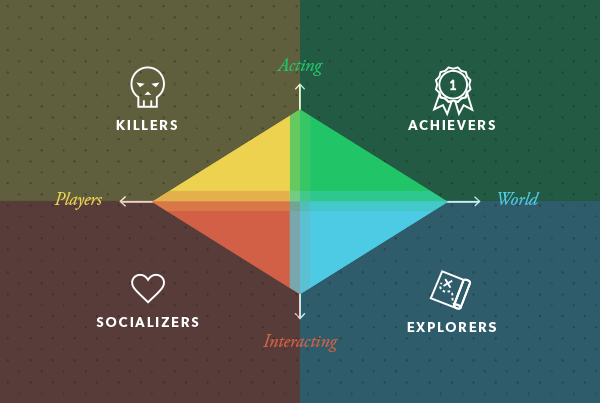
\includegraphics[width=0.5\textwidth]{images/TypeOfPlayersBartle.png}
  \caption[Caption for LOF]{Real caption\footnotemark}
  \label{fig:Players}
\end{figure}

\footnotetext{Source: \url{http://www.example.com/theimage.png}}

\section{Definicion}

Hoy en dia \emph{gamification} se ha convertido en una herramienta para las empresas 
para poder captar mas clientes. Cada dia aumenta el uso de este concepto por lo que es
necesario entregar una definicion apropiada para el concepto.  \emph{Gamification} se puede definir
como "el uso de elementos del dise�o de juego en contextos diferentes al de juego". Para entender mejor 
los conceptos bajo esta definicion se explicara por partes:

\begin{itemize}

\item Juego: En primer lugar este concepto se refiere al juego, en su todo, y no a la accion de jugar.
	Este concepto es caracterizado por un conjunto de reglas explicitas que crean un ambiente 
	en donde los jugadores buscan la competicion para completar objetivos y metas.

	This relates to \emph{games} and not to \emph{play}. The idea of game is
characterized by explicit rules that make a context where the competition or strife
of actors let them go towars goals or achievements.    

\item Elementos del dise�o de juego: Dentro de este concepto se puede encontrar 2 definiciones.
	La primera, es una definicion estricta que solo acepta ciertos elementos unicos. La 
	segunda, es una definicion en donde todos los elementos pueden ser utilizados. Para llegar a una
	definicion robusta es necesario juntar ambas y asi obtener un conjunto mas restrictivo en donde
	los elementos a utilizar son carateristicos a los juegos, que se encuentran en la mayoria de estos y
	que cumplen una rol importante en la jugabilidad de estos.

\item Contextos diferentes al de juego: Este es el concepto mas complejo de explicar debido a que es una idea 
	abstracta. Una forma de explicarla es como una situacion de la vida cotidiana que existe fuera
	de un juego o de un ambiente que contiene \emph{gamification}.
	

